% License: CC BY-SA
% Authors: See authors below and see also acknowledgement for authors of some images or research

\documentclass[25pt, margin=0mm, innermargin=15mm, blockverticalspace=15mm, colspace=15mm, subcolspace=8mm]{tikzposter}
\geometry{paperwidth=48in,paperheight=36in}

% to stretch boxes over whole paper with custor paper size
\makeatletter
\setlength{\TP@visibletextwidth}{\textwidth-2\TP@innermargin}
\setlength{\TP@visibletextheight}{\textheight-2\TP@innermargin}
\makeatother


\usepackage[utf8]{inputenc}
\usepackage{wrapfig}
\usepackage[hidelinks]{hyperref}

% For bibliography styling
%% TODO: all names should be abbreviated
\usepackage{natbib}


% \definecolor{textcolor}{HTML}{000000}
%
% \definecolor{titleTextColor}{HTML}{009000}
% \definecolorpalette{grassColorPalette} {
%   \definecolor{colorOne}{HTML}{419041}
%   % \definecolor{colorTwo}{HTML}{cccccc}
%   \definecolor{colorTwo}{HTML}{dddddd}
%   \definecolor{colorThree}{HTML}{F1B52D}
%   % \definecolor{colorThree}{HTML}{EFA126}
% }
%
% \usetheme{Rays}
% \usecolorstyle[colorPalette=grassColorPalette]{Britain}

\definecolor{titleTextColor}{HTML}{000000}

\definecolor{textcolor}{HTML}{000000}
\definecolor{viridisYellow}{HTML}{C1DF24}
\definecolor{viridisViolet}{HTML}{482173}
\definecolor{viridisGreen}{HTML}{51C46B}
\definecolor{viridisBlueGreen}{HTML}{209C8B}

\definecolorpalette{grassColorPalette} {
  \definecolor{colorOne}{HTML}{38588C}
  \definecolor{colorTwo}{HTML}{dddddd}
  \definecolor{colorThree}{named}{viridisYellow}
}

\usetheme{Default}
\usecolorstyle[colorPalette=grassColorPalette]{Britain}

\colorlet{backgroundcolor}{white}
\colorlet{framecolor}{viridisGreen!90!black}
\colorlet{blocktitlebgcolor}{viridisGreen!90!black}
% \colorlet{framecolor}{viridisGreen}
% \colorlet{blocktitlebgcolor}{viridisGreen}
\colorlet{blocktitlefgcolor}{white}

\title{
\begin{minipage}{\linewidth}
\centering
\vspace*{-0.25\grasslogoheight}
\Huge
\textcolor{titleTextColor}{
\textsf{\textbf{
\fontsize{85}{60}\selectfont
Generalized 3D fragmentation index derived from lidar point clouds
}}
}
\end{minipage}
}

\newlength{\grasslogoheight}
\setlength{\grasslogoheight}{0.07\textheight}
\newlength{\instlogoheight}
\setlength{\instlogoheight}{0.33\grasslogoheight}

\titlegraphic{
\begin{minipage}{0.3\linewidth}
\vspace{0.6\grasslogoheight}
\hspace{0.1\grasslogoheight}

\includegraphics[height=\grasslogoheight]{ncsu-cnr}
\vspace{0.25\grasslogoheight}
\end{minipage}
\hfill
\begin{minipage}{0.3\linewidth}
\setlength{\baselineskip}{120pt}
\begin{flushright}
\vspace{0.6\grasslogoheight}
\hspace*{-0.6\grasslogoheight}

\includegraphics[height=0.8\grasslogoheight]{cga}
\hspace{0.1\grasslogoheight}
\end{flushright}
\end{minipage}
\vspace{-1.6\grasslogoheight}
}

% \setlength{\blocktitleheight}{0.02\textheight}

% style for institute numbers
\newcommand{\inst}[1]{\hspace{2pt}$^{\mbox{\normalsize#1}}$\hspace{-7pt}}
\newcommand{\instlist}[1]{\hspace{1pt}$^{\mbox{\normalsize#1}}$\hspace{2pt}}

\author{
Vaclav Petras\inst{1},
Douglas J. Newcomb\inst{2,*},
and Helena Mitasova\inst{1,3}
}
\institute{
\large
\instlist{1}North Carolina State University, Center for Geospatial Analytics (wenzeslaus@gmail.com, vpetras@ncsu.edu)\\
\instlist{2}U.S. Fish and Wildlife Service, Raleigh;
\instlist{*}The findings do not necessarily represent the views of the USFWS.\\
\instlist{3}North Carolina State University, Department of Marine, Earth, and Atmospheric Sciences
}

\hypersetup
{
    pdfauthor={V. Petras, D. J. Newcomb, H. Mitasova},
    pdfsubject={Poster and visual abstract for the paper of the same name (Petras et al. 2017)},
    pdftitle={Generalized 3D fragmentation index derived from lidar point clouds},
    pdfkeywords={3D raster, voxel model, spatial pattern, lidar, raster algebra, spatial indices}
}

% \usetemplate{1}
% \setinstituteshift{1}

% \setblocktitleheight{2}
% \setblockspacing{1}

\graphicspath{{images/}{logos/}}

\newcommand{\blocktitlewrap}[1]{\textsf{\textbf{\huge#1}}}
% it is not possible (?) to change block title in the class, using wrapper
% the command introduced using:
%   sed -i 's/\\block{\([^}]*\)}/\\block{\\blocktitlewrap{\1}}/g' main.tex

% GRASS module
\newcommand{\gmodule}[1]{\href{http://grass.osgeo.org/grass72/manuals/#1.html}{\emph{#1}}}
\newcommand{\gamodule}[1]{\href{http://grass.osgeo.org/grass72/manuals/addons/#1.html}{\emph{#1}}}
\newcommand{\gmodulenolink}[1]{\emph{#1}}

\begin{document}

\maketitle[width=.976\textwidth]
% \maketitle
% \addlogo[north west]{(2,-1)}{9cm}{images/Grass_GIS}
%Please insert your institution logo here
% \addlogo[north east]{(-2,-2.5)}{4cm}{images/logo_FEM_CRI}
% \addlogo[north east]{(-2,-5.5)}{4cm}{images/NC_State_Seal}
% \addlogo[north east]{(-8,-2.5)}{4cm}{images/Logo_cvut}
% \addlogo[north east]{(-8,-6.5)}{4cm}{images/IWMI_logo}
% \addlogo[north east]{(-2,-10.5)}{4cm}{images/logo_ec-jrc}

\begin{columns}

%%%%%%%%%%%%%%%%%%%%%%%%%%%%%%%%%%%%%%%%%%%%%%%%%%%%%%%%%%%%%%%%%%%%%
%%%%%%%%%%%%%%%%%%%%%%%%%%%%%%%%%%%%%%%%%%%%%%%%%%%%%%%%%%%%%%%%%%%%%
%%%%%%%%%%%%%%%%%%%%%%%%%%%%%%%%%%%%%%%%%%%%%%%%%%%%%%%%%%%%%%%%%%%%%
%%%%%%%%%%%%%%%%%%%%%%%%%%%%%%%%%%%%%%%%%%%%%%%%%%%%%%%%%%%%%%%%%%%%%
\column{0.25}

%%%%%%%%%%%%%%%%%%%%%%%%%%%%%%%%%%%%%%%%%%%%%%%%%%%%%%%%%%%%%%%%%%%%%%%%%%%%%%%%
% \block{\blocktitlewrap{Highlights}}
% {
% % \setlength{\parskip}{0.3ex}
%
% \renewcommand{\labelitemi}{\textcolor{gray}{$\bullet$}\hspace{0.5ex}}
% \newcommand{\blocksectiontitle}[1]{\bigskip\textbf{\textcolor{gray}{\textsf{#1}}}}
%
% \blocksectiontitle{Poster topic highlights}
%
% \begin{itemize}
%  \item Algorithms and models included in GRASS GIS remain available long term \citep{chemin2015grass}.
%  \item Analytical tools are not limited to one domain but spread across many fields.
%  \item New tools can be built based on functionality or code of the existing ones
%        regardless of the particular domain of problems they belong to.
%  \item Both the functionality and the code are evaluated
%        by the community of users and developers in different fields and scales.
% % continuous automated tests (Petras, 2014 \cite{Petras2014}),
% \end{itemize}
%
% }


%%%%%%%%%%%%%%%%%%%%%%%%%%%%%%%%%%%%%%%%%%%%%%%%%%%%%%%%%%%%%%%%%%%%%
\block{\blocktitlewrap{Introduction \& Data}}{

Point clouds with increased point densities create new opportunities
for analyzing landscape structure in 3D space.
Taking advantage of currently acquired dense point clouds
we have extended a 2D forest fragmentation index developed for regional scale analyses \citep{riitters2000global}
into a 3D index for analyzing vegetation structure at a much finer scale.
We applied this method to a point cloud obtained by airborne lidar capturing
a suburban area with mixed forest cover.

\vspace{2ex}

\begin{center}
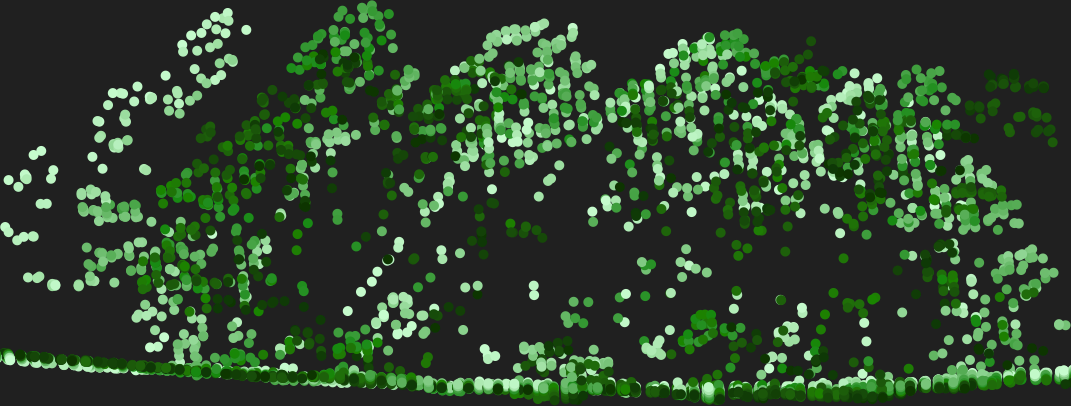
\includegraphics[width=\linewidth]{lidar_profile}
\end{center}

Profile (transect) of a multiple-return lidar point cloud in a forested area
showing captured tree structure.

\vspace{3ex}

\begingroup
\centering
\begin{minipage}{0.36\linewidth}
\centering
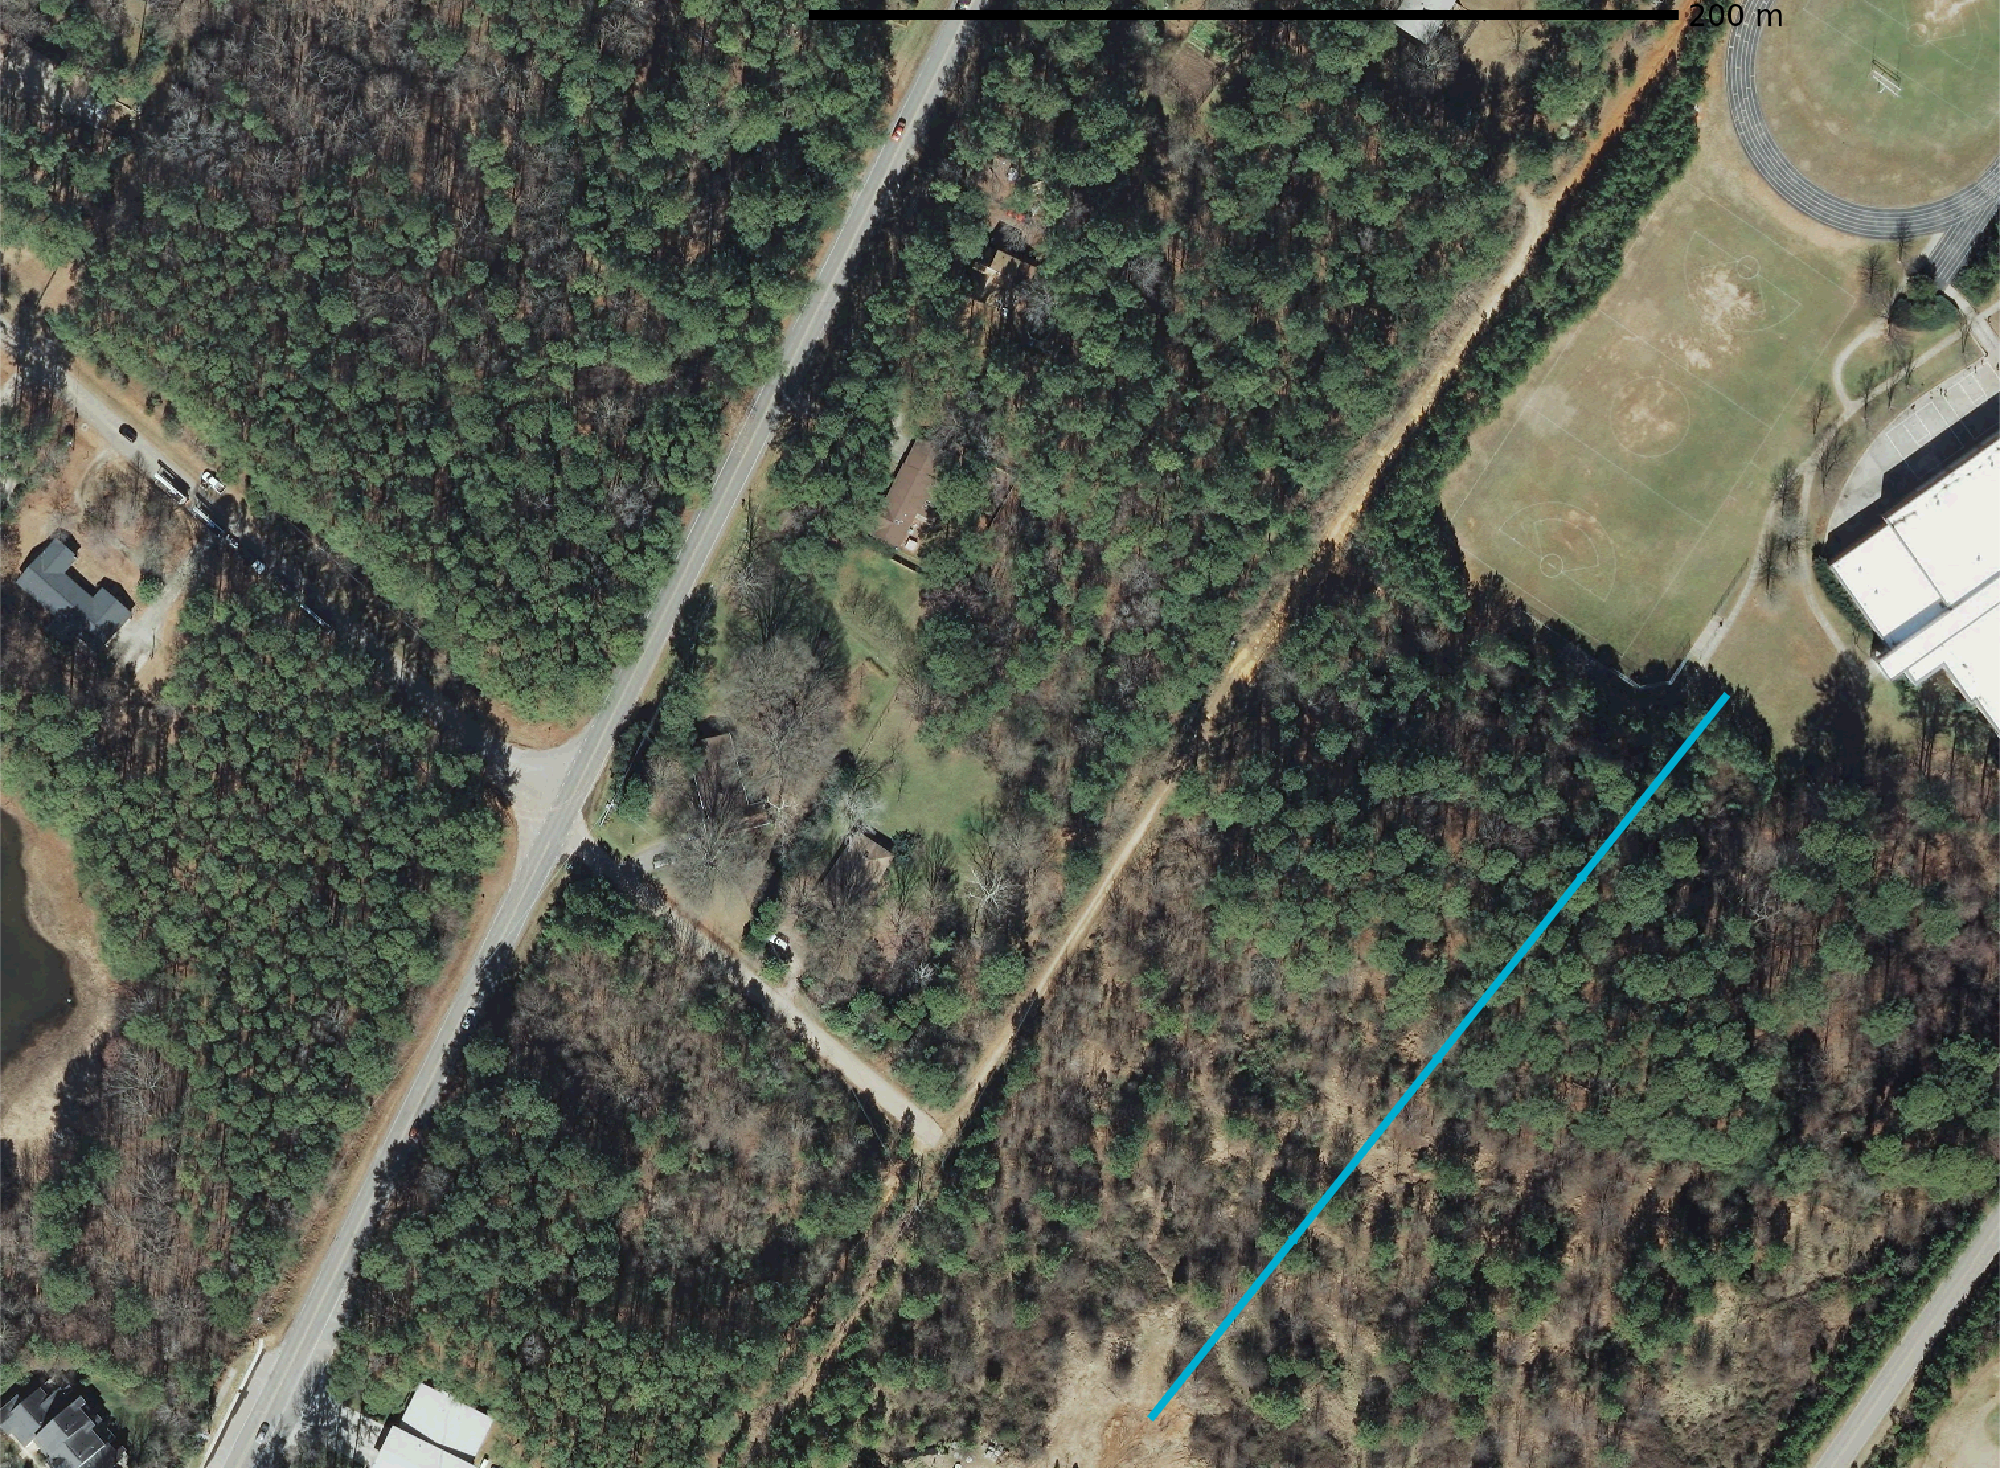
\includegraphics[width=\textwidth]{ortho}
\end{minipage}
~
\begin{minipage}{0.60\linewidth}
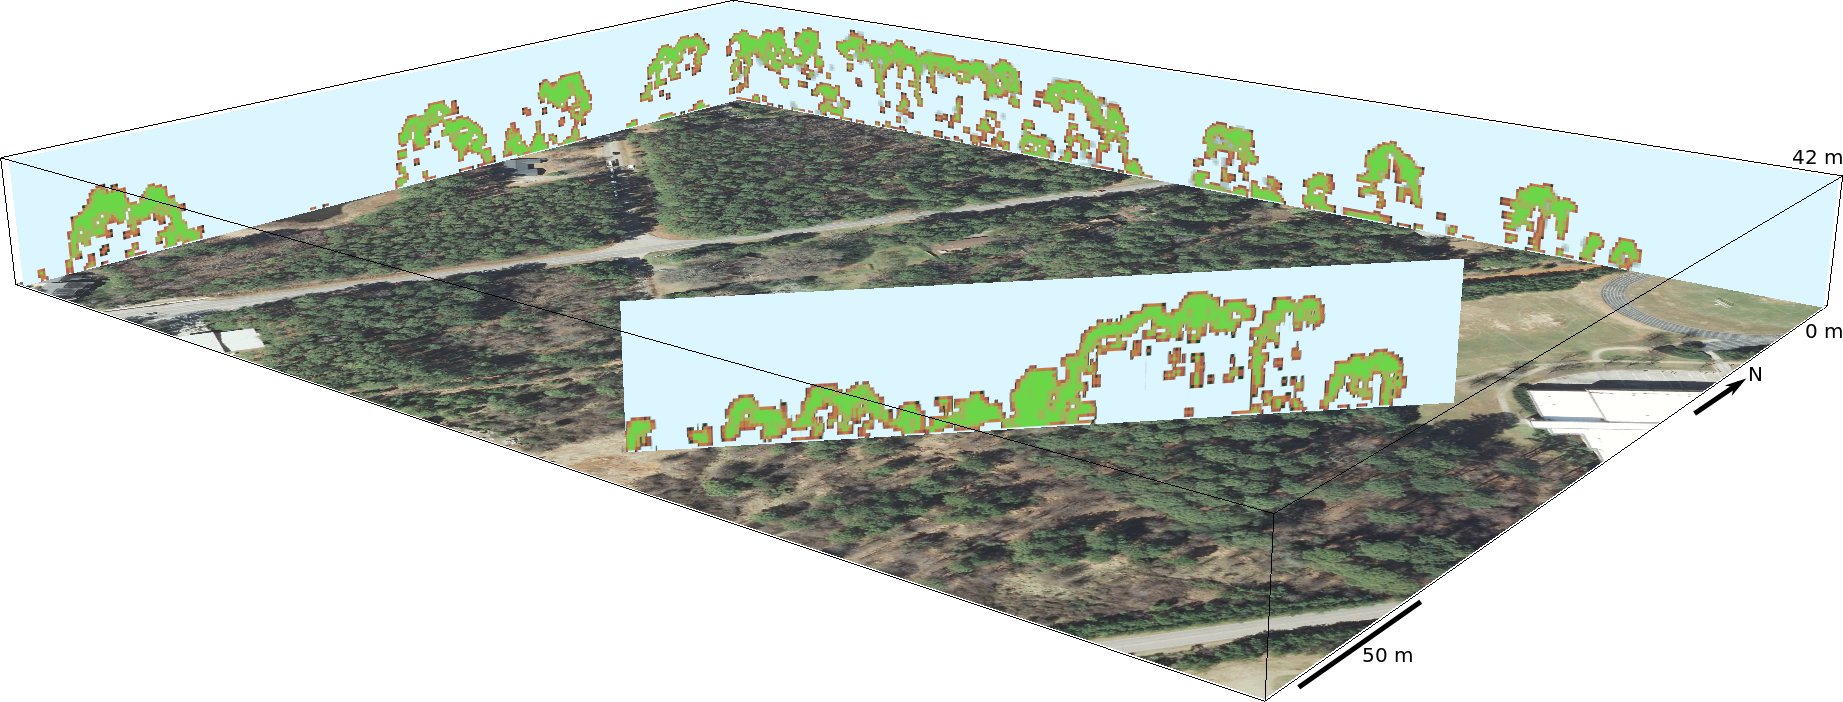
\includegraphics[width=\textwidth]{profile3d}
\end{minipage}
\endgroup

\bigskip

% \begin{minipage}{0.96\linewidth}
Orthophoto of the study area near Centennial Campus Middle School, Raleigh, North Carolina (left)
% \end{minipage}
% ~
% \begin{minipage}{0.60\linewidth}
% \centering
and 3D representation of a point cloud processed by the presented method (right).
% \end{minipage}

}

%%%%%%%%%%%%%%%%%%%%%%%%%%%%%%%%%%%%%%%%%%%%%%%%%%%%%%%%%%%%%%%%%%%%%
\block{\blocktitlewrap{3D Raster}}{

We processed the lidar point cloud using a set of 3D raster methods
including 3D raster algebra.
Although this technique is rarely applied in the geospatial field,
it is as straightforward to use as well-established 2D raster and image processing methods.

\vspace{2ex}

\begingroup
\centering
\begin{minipage}{0.47\linewidth}
\centering
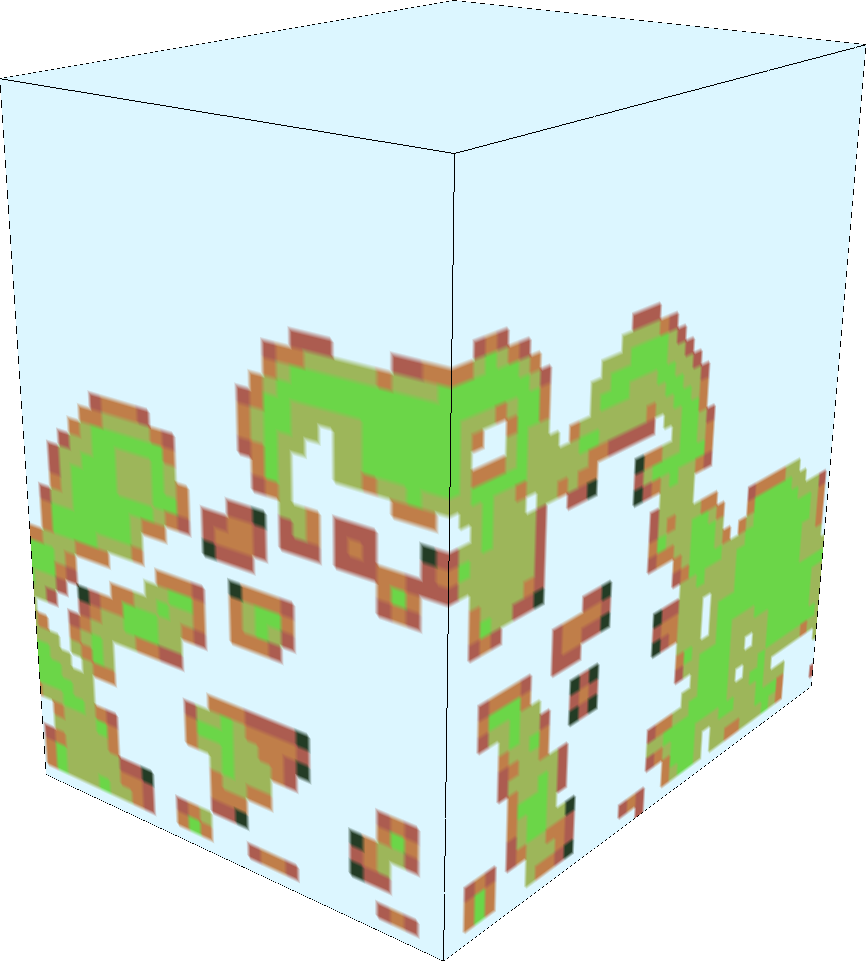
\includegraphics[width=\textwidth]{raster3d}
\end{minipage}
~
\begin{minipage}{0.47\linewidth}
\centering
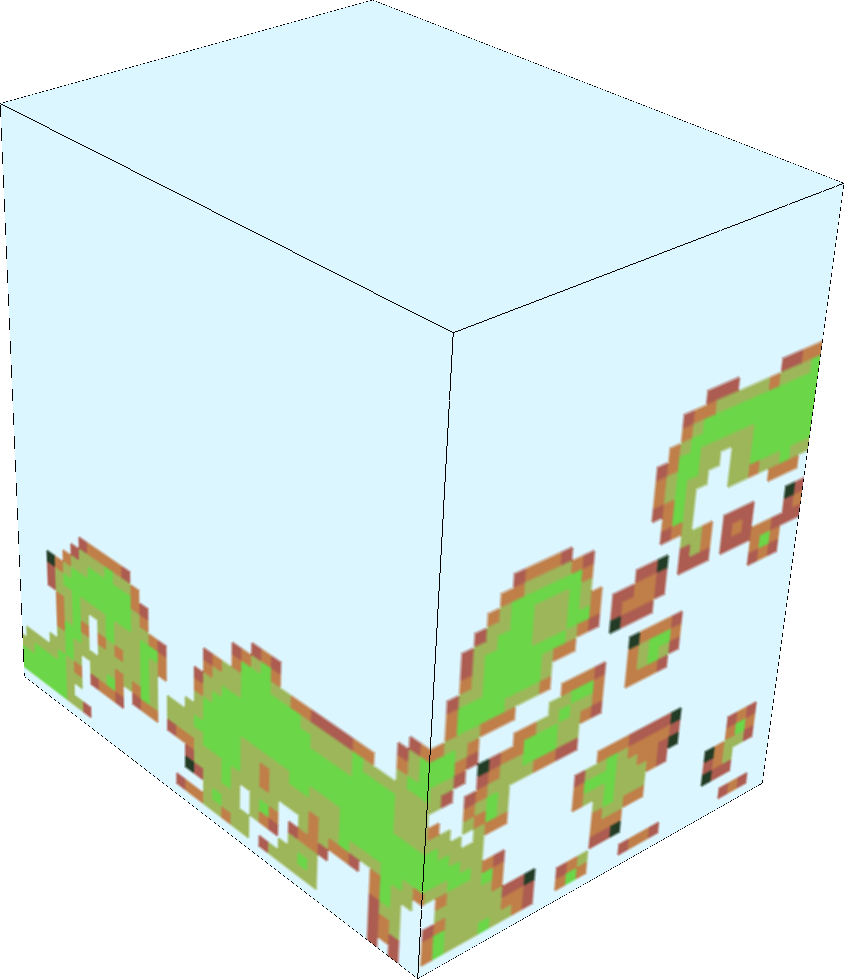
\includegraphics[width=\textwidth]{raster3d_2}
\end{minipage}
\endgroup

\bigskip

% \begin{minipage}{0.96\linewidth}
An example 3D raster which represents the 3D fragmentation index.
It is a small sample of size 33$\times$44$\times$46 3D cells
in one position (left) and then rotated (right).
% \end{minipage}
% ~
% \begin{minipage}{0.48\linewidth}
% \centering
% \end{minipage}

}


%%%%%%%%%%%%%%%%%%%%%%%%%%%%%%%%%%%%%%%%%%%%%%%%%%%%%%%%%%%%%%%%%%%%%
%%%%%%%%%%%%%%%%%%%%%%%%%%%%%%%%%%%%%%%%%%%%%%%%%%%%%%%%%%%%%%%%%%%%%
%%%%%%%%%%%%%%%%%%%%%%%%%%%%%%%%%%%%%%%%%%%%%%%%%%%%%%%%%%%%%%%%%%%%%
%%%%%%%%%%%%%%%%%%%%%%%%%%%%%%%%%%%%%%%%%%%%%%%%%%%%%%%%%%%%%%%%%%%%%
\column{0.25}

%%%%%%%%%%%%%%%%%%%%%%%%%%%%%%%%%%%%%%%%%%%%%%%%%%%%%%%%%%%%%%%%%%%%%
\block{\blocktitlewrap{3D Fragmentation Index}}{

The 3D fragmentation index is based on \cite{riitters2000global}
and uses presence, absence, and configuration of lidar points in cells in a moving window.
The index is based on classification of $P_f$ and $P_{f\!f}$ values.
The $P_f$ value is computed as a ratio of occupied cells
(the y-axis direction in the figure below)
and the $P_{f\!f}$ value is computed as a ratio of fully versus partially occupied cell pairs
(the x-axis direction in the figure below).

\vspace{5ex}

\begin{minipage}{0.48\linewidth}
\centering
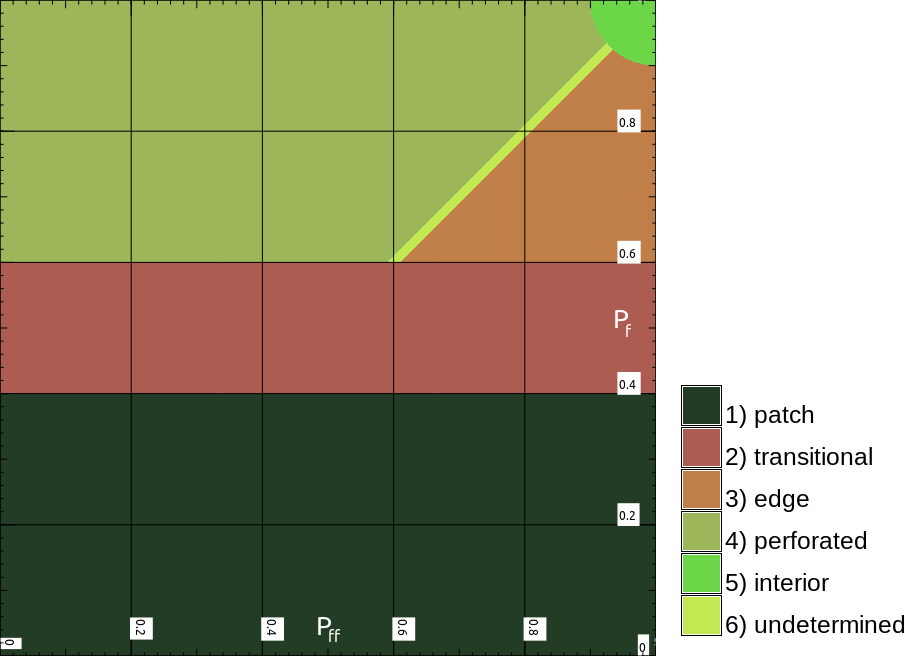
\includegraphics[width=\textwidth]{index_values_pf_pff}
\end{minipage}
~
\begin{minipage}{0.48\linewidth}
\centering

\includegraphics[width=\textwidth]{zonal_plot_n_pf_pff_zone_1}
\end{minipage}

\bigskip

\begin{minipage}{0.48\linewidth}
Classification schema of $P_f$ and $P_{f\!f}$ components to the fragmentation index.
\end{minipage}
~
\begin{minipage}{0.48\linewidth}
Relation of $P_f$ and $P_{f\!f}$ index components to the number of points per cell
(zone 1).
% Example of the index and color table applied to the data from the study area
\end{minipage}

\vspace{4ex}

\begin{center}
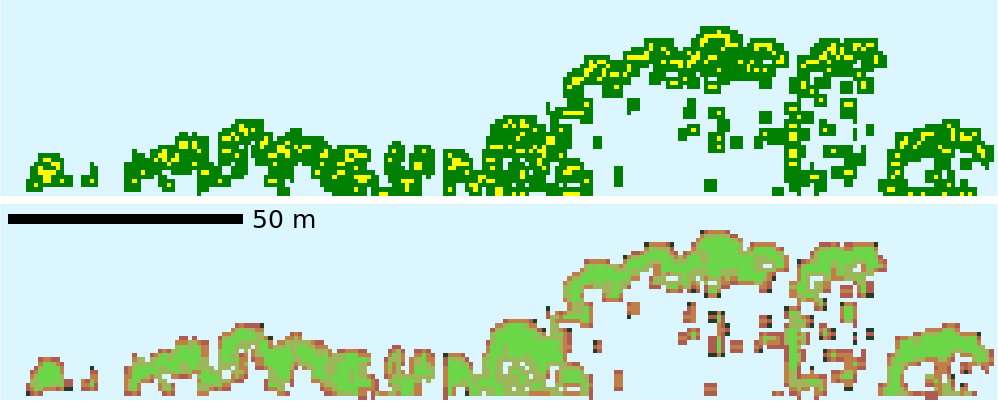
\includegraphics[width=\linewidth]{profiles}
\end{center}

A selected profile (vertical slice) of 3D raster representing
the reconstructed 3D vegetation structure (top)
and fragmentation index profile (bottom).



\vspace{4ex}

\begin{center}
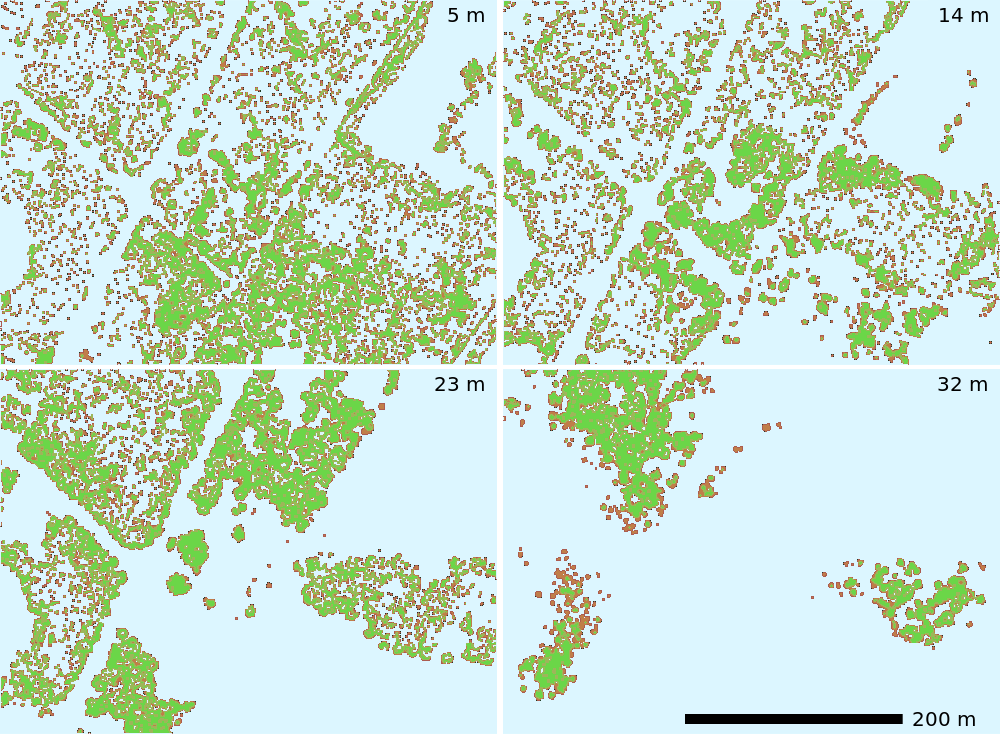
\includegraphics[width=\linewidth]{hslice}
\end{center}

Horizontal slices of the 3D fragmentation index.
Each image shows a horizontal slice for a given height.
The used colors are defined above with addition of light blue color for exterior.
% The areas in the north and north-east show only limited number
% of interior and a lot of transitional and edge class for the lower heights,
% while for the higher height a lot of interior and perforated class is visible.
%       The edges of these areas behave similarly with interior coming and disappearing sooner
%       indicating lower vegetation but with the same vertical structure.
% This is different from the area in the south-east corner with a lot of
% interior in the lowest levels but only exterior in the higher levels indicating
% dense low vegetation.



}

%%%%%%%%%%%%%%%%%%%%%%%%%%%%%%%%%%%%%%%%%%%%%%%%%%%%%%%%%%%%%%%%%%%%%
%%%%%%%%%%%%%%%%%%%%%%%%%%%%%%%%%%%%%%%%%%%%%%%%%%%%%%%%%%%%%%%%%%%%%
%%%%%%%%%%%%%%%%%%%%%%%%%%%%%%%%%%%%%%%%%%%%%%%%%%%%%%%%%%%%%%%%%%%%%
%%%%%%%%%%%%%%%%%%%%%%%%%%%%%%%%%%%%%%%%%%%%%%%%%%%%%%%%%%%%%%%%%%%%%
\column{0.25}


%%%%%%%%%%%%%%%%%%%%%%%%%%%%%%%%%%%%%%%%%%%%%%%%%%%%%%%%%%%%%%%%%%%%%
\block{\blocktitlewrap{Results}}{

The index can be used to describe different types
of vegetation structure in 3D (first poster column) and in 2D (this column).

\vspace{2.5ex}

\begin{center}
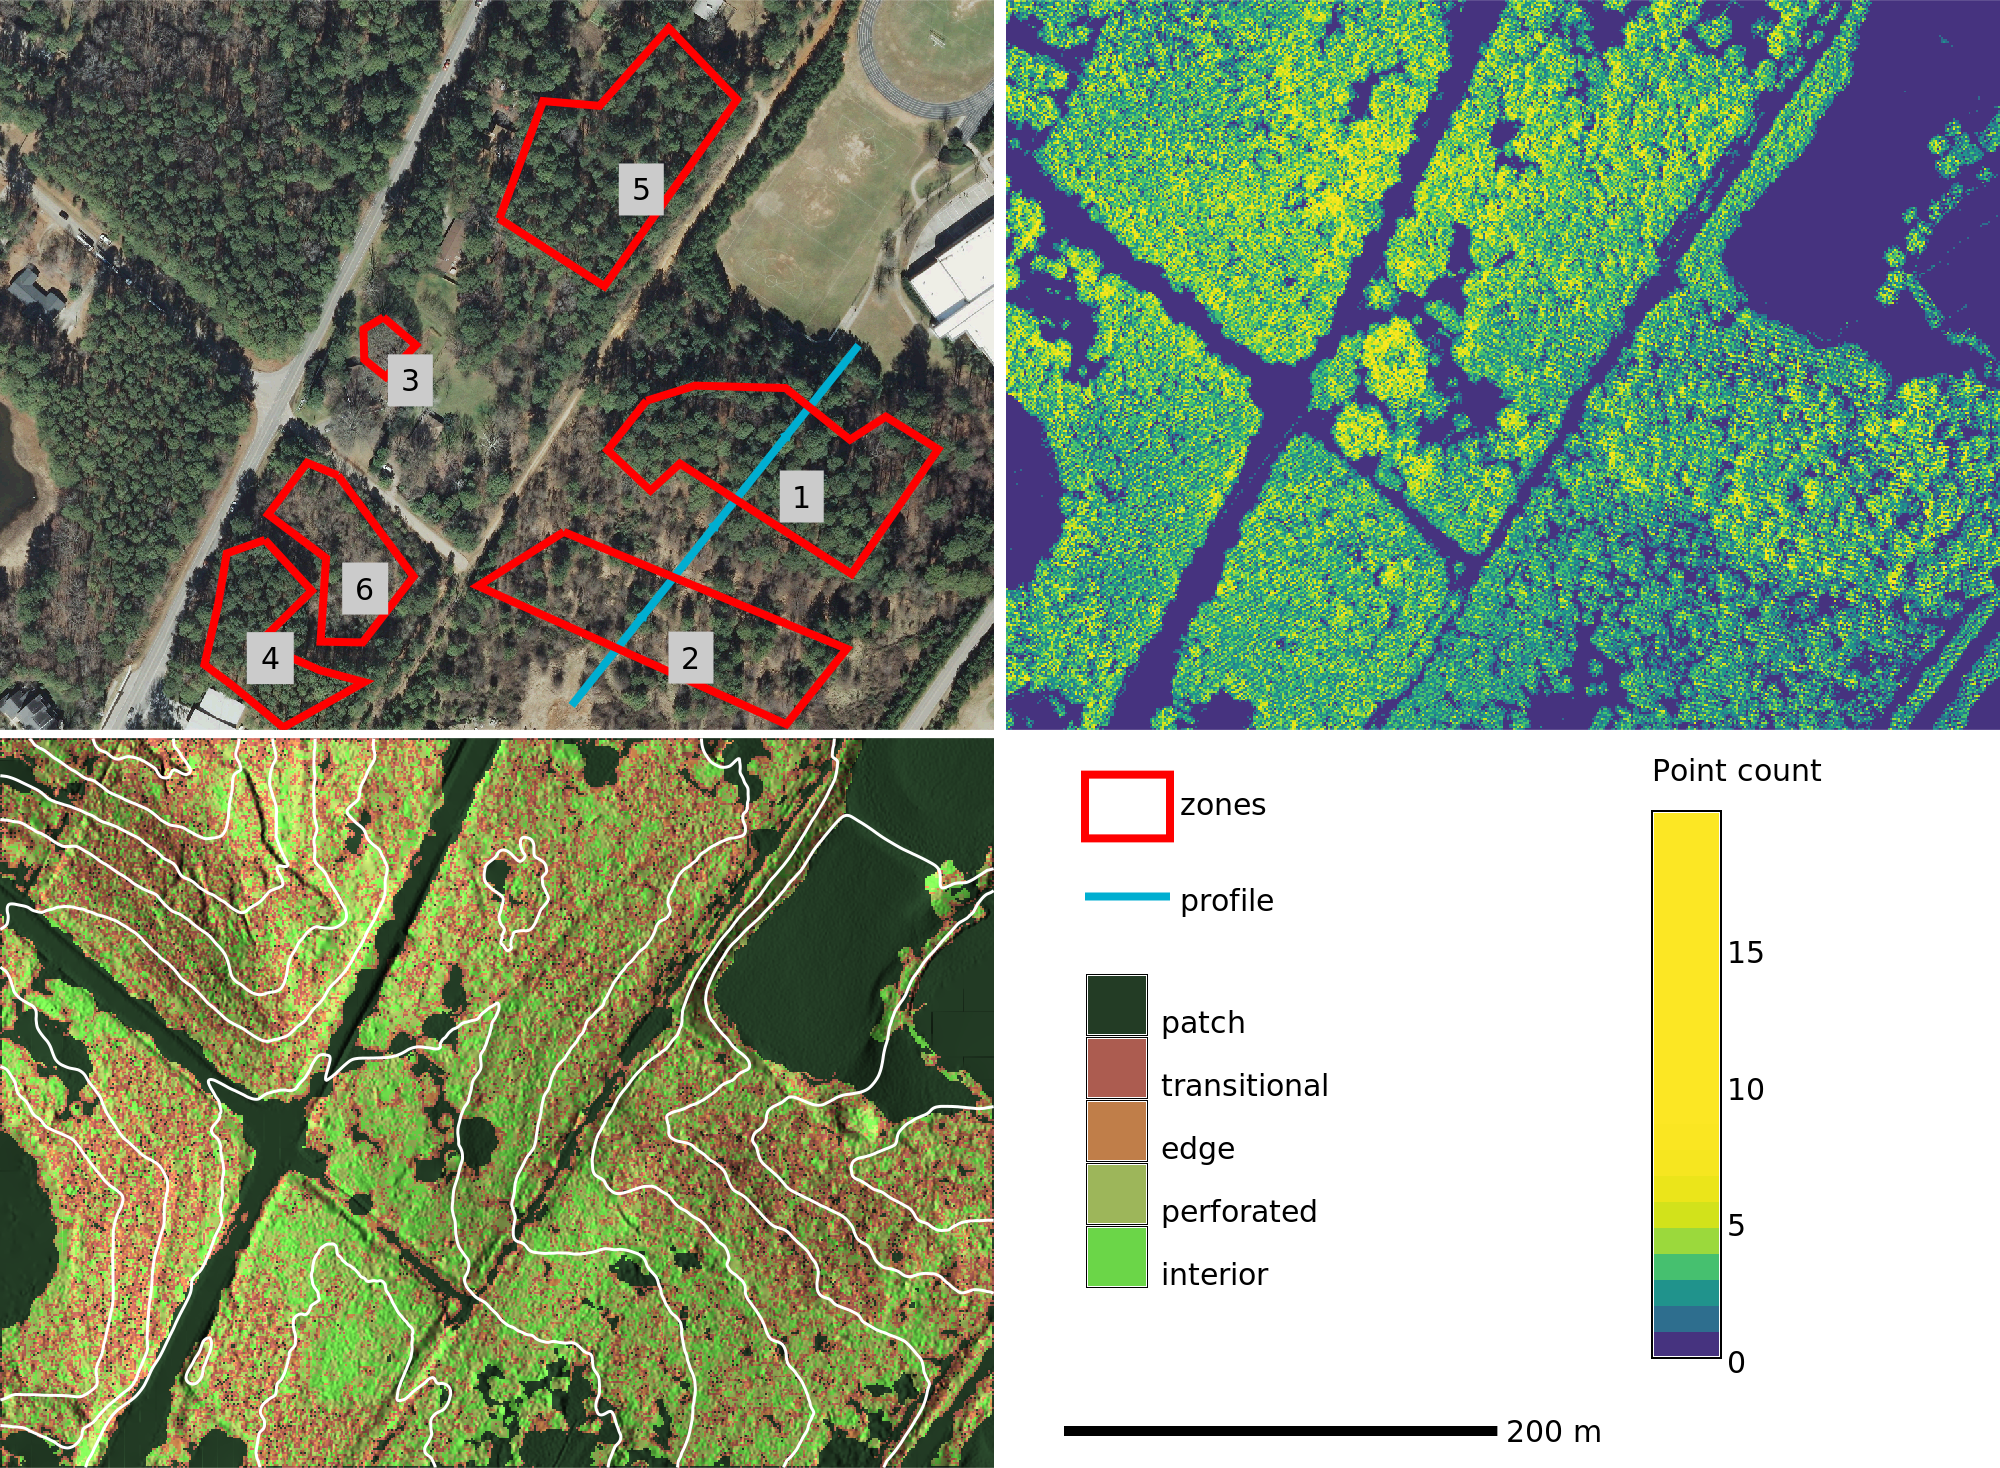
\includegraphics[width=\linewidth]{comparison_ortho}
\end{center}

The index (bottom left) detects vegetation structure beyond what is visible
from the point density (top right).

\vspace{2.5ex}

\begin{center}
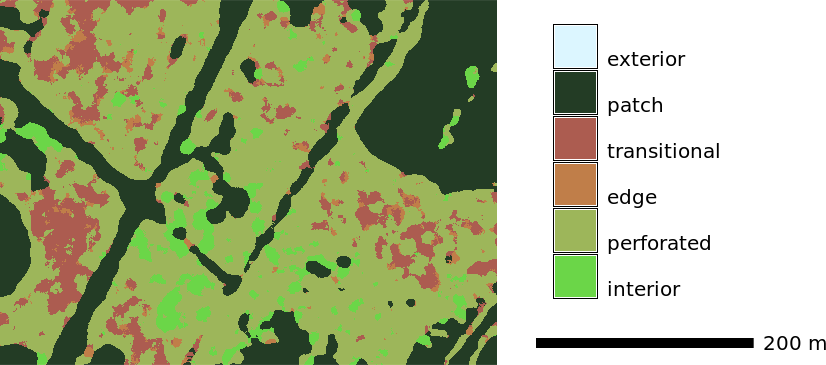
\includegraphics[width=\linewidth]{main_category}
\end{center}

Dominant fragmentation class in each vertical column characterizes
number of distinct zones in the study area.

\vspace{2.5ex}

\begin{center}
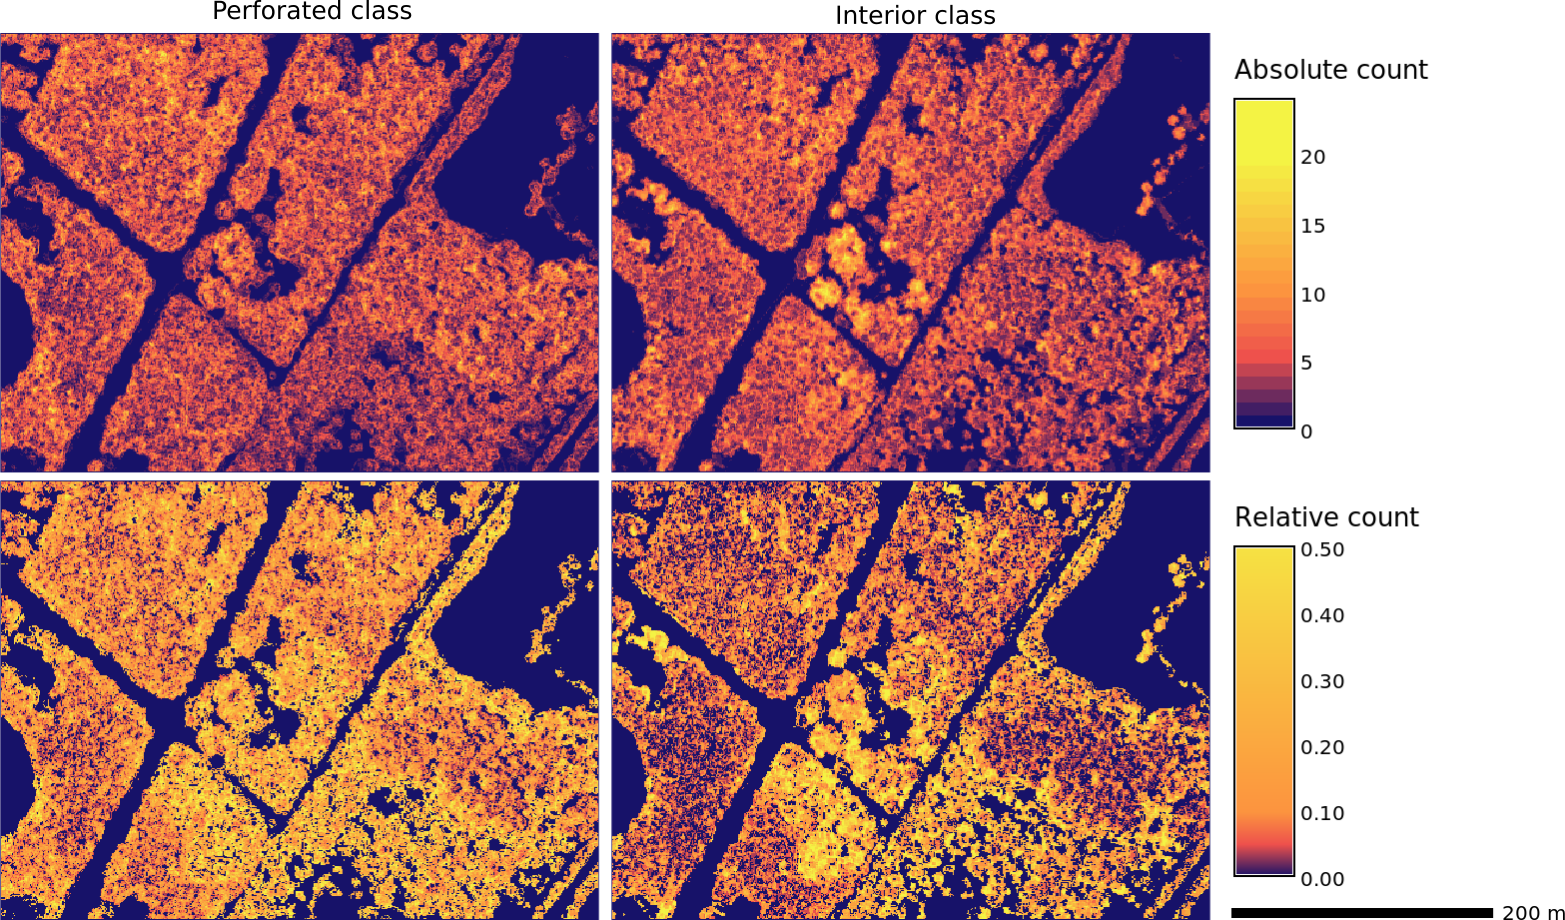
\includegraphics[width=\linewidth]{counts_all}
\end{center}

The absolute count of interior cells shows
the whole south-east quadrant as mostly homogeneous (top right)
while the relative count, i.e. percentage in vertical column, shows it as two distinct
vegetation types (bottom right).
The relative count of perforated cells (bottom left) also suggest
greater distinction of individual vegetation types.

}

%%%%%%%%%%%%%%%%%%%%%%%%%%%%%%%%%%%%%%%%%%%%%%%%%%%%%%%%%%%%%%%%%%%%%
%%%%%%%%%%%%%%%%%%%%%%%%%%%%%%%%%%%%%%%%%%%%%%%%%%%%%%%%%%%%%%%%%%%%%
%%%%%%%%%%%%%%%%%%%%%%%%%%%%%%%%%%%%%%%%%%%%%%%%%%%%%%%%%%%%%%%%%%%%%
%%%%%%%%%%%%%%%%%%%%%%%%%%%%%%%%%%%%%%%%%%%%%%%%%%%%%%%%%%%%%%%%%%%%%
\column{0.25}

%%%%%%%%%%%%%%%%%%%%%%%%%%%%%%%%%%%%%%%%%%%%%%%%%%%%%%%%%%%%%%%%%%%%%
\block{\blocktitlewrap{Open Science}}{

% \setlength{\parskip}{0.3ex}

\renewcommand{\labelitemi}{\textcolor{gray}{$\bullet$}\hspace{0.5ex}}
% \newcommand{\blocksectiontitle}[1]{\bigskip\textbf{\textcolor{gray}{\textsf{#1}}}}

% \blocksectiontitle{Poster topic highlights}

\begin{itemize}
 \item Source code for all the presented methods is provided.
 \item The 3D fragmentation index is implemented as a GRASS GIS module \citep{neteler2012grass}.
 \item The module is published in the GRASS GIS Addons repository
       alongside tools from other scientists \citep{chemin2015grass}.
 \item Helper tools such as the one for profiles were also implemented as GRASS GIS modules and published.
 \item We prepared a publicly available Git repository hosted on GitHub
       which contains the data for the study area, scripts to perform the analyses presented here,
       and details about the dependencies.
 \item Using Docker, this repository can be turned into a complete runtime environment
       to produce the figures and underlying data for this manuscript \citep{boettiger2015introduction}.
 \item We also connected the repository with a continuous integration service, Travis CI,
       which will show if the basic functionality was broken by any future changes.
 \item We leveraged and reviewed existing functionality and code in GRASS GIS.
 \item Algorithms and models included in GRASS GIS remain available long term \citep{petras2017innovations}.
\end{itemize}

}

%%%%%%%%%%%%%%%%%%%%%%%%%%%%%%%%%%%%%%%%%%%%%%%%%%%%%%%%%%%%%%%%%%%%%
\block{\blocktitlewrap{References}}{

\newcommand{\blocksectiontitle}[1]{\bigskip\textbf{\textcolor{gray}{\textsf{#1}}}}
% \newcommand{\blocksectiontitle}[1]{\textbf{#1}}

\newcommand{\listhspace}{\hspace{0.005\linewidth}}
\newcommand{\listlogowidth}{0.10\linewidth}
\newcommand{\listtextwidth}{0.89\linewidth}

%%%%%%%%%%%%%%%%%%%%%%%%%%%%%%%%%%%%%%%%%%%%%%%%%%%%%%%%%%%%%%%%%%%%%
\blocksectiontitle{Literature}
\begingroup
\scriptsize
\renewcommand{\section}[2]{}%
\bibliographystyle{apalike}
\bibliography{poster}
\endgroup


%%%%%%%%%%%%%%%%%%%%%%%%%%%%%%%%%%%%%%%%%%%%%%%%%%%%%%%%%%%%%%%%%%%%%
\blocksectiontitle{Paper (How to Cite This Work)}

\smallskip

\begingroup

\begin{minipage}{\listlogowidth}
\centering

\includegraphics[width=0.9\linewidth]{open_access}
\end{minipage}
\listhspace
\begin{minipage}{\listtextwidth}
Petras, Vaclav, Douglas J. Newcomb, and Helena Mitasova.
"Generalized 3D fragmentation index derived from lidar point clouds."
\textit{Open Geospatial Data, Software and Standards}
2, no. 1 (2017): 9.

\url{https://doi.org/10.1186/s40965-017-0021-8}
\end{minipage}

\endgroup

%%%%%%%%%%%%%%%%%%%%%%%%%%%%%%%%%%%%%%%%%%%%%%%%%%%%%%%%%%%%%%%%%%%%%
\blocksectiontitle{Acknowledgements}

\smallskip

\begin{minipage}{\listlogowidth}
\centering

\includegraphics[width=0.9\linewidth]{grass}
\end{minipage}
\listhspace
\begin{minipage}{\listtextwidth}
We are grateful to the GRASS GIS developer and user community for developing, extending, and maintaining
the GRASS GIS software package.
We further acknowledge Emmanuel Sambale, Stefan Sylla, and Paulo van Breugel
who originally implemented the forest fragmentation index in GRASS GIS.
\end{minipage}

% \bigskip
%
% \begin{minipage}{\listlogowidth}
% \includegraphics[width=\linewidth]{osgeo}
% \end{minipage}
% \listhspace
% \begin{minipage}{\listtextwidth}
% We acknowledge Open Source Geospatial Foundation (OSGeo)
% which provides infrastructure for GRASS GIS project
% and its user-contributed scientific modules.
% \end{minipage}

\vspace{0.3cm}

\textcolor{gray}{
\hrulefill
}

\vspace{0.1cm}

\newcommand{\qrcodesize}{0.05\linewidth}

% qrencode http://grass.osgeo.org -o qr_grass.eps -t EPS
% epspdf -b qr_grass.eps qr_grass.pdf

\begin{center}
\begin{tabular}{c}

% \hspace{5mm}

% \begin{minipage}{\qrcodesize}
% \includegraphics[width=\textwidth]{./images/qr_grass.pdf}
% \end{minipage}
% ~
% \begin{minipage}{0.25\linewidth}
% \small {\href{http://grass.osgeo.org}{\nolinkurl{grass.osgeo.org}}}
% \end{minipage}

\begin{minipage}{0.1\linewidth}
\href{http://creativecommons.org/licenses/by-sa/4.0/}{
\includegraphics[width=\textwidth]{ccbysa}}
\end{minipage}
~
\begin{minipage}{0.7\linewidth}
\small This poster is licensed under a Creative Commons Attribution-ShareAlike 4.0 International License.
\end{minipage}

\end{tabular}
\end{center}

\vspace{-0.08cm}
}





\end{columns}

\end{document}
